\chapter{Use applicable action in start -ai}

Aim of this operation is to find actions that are applicable in init, do not destroy possibility of applying another action and can be used at most once; once such action is found, is applied to init and removed from SAS. 

\begin{figure}
	\begin{subfigure}[b]{0.4\textwidth}
		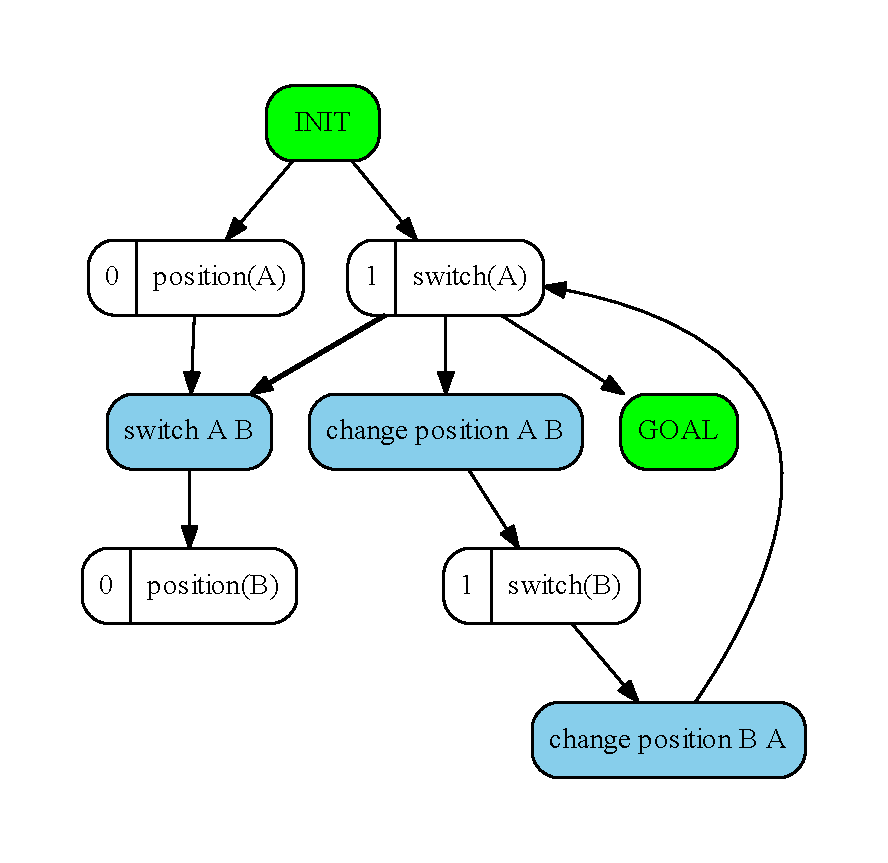
\includegraphics[scale=0.4]{useApplicableActionInStart/figures/applyOnlyOne_input}
		\caption{before reduction}
	\end{subfigure}	
	\begin{subfigure}[b]{0.4\textwidth}
		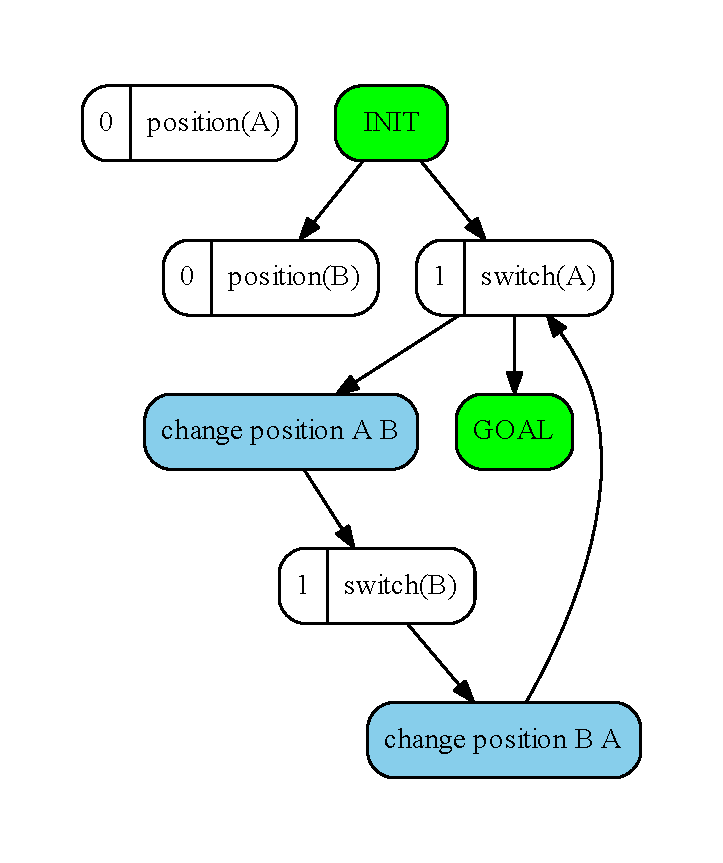
\includegraphics[scale=0.4]{useApplicableActionInStart/figures/applyOnlyOne_output}
		\caption{after reduction}
	\end{subfigure}
	\caption{Action \emph{switch A B} can be applied in init, is applicable at most once and does not destroy application of other actions. Action \emph{change B A} is not applicable in init. Action \emph{changes A B} is applicable in init but it may be applied more than once and its application destroys usage of \emph{switch A B}.}		
\end{figure}


\section{Reduce operation}
Let's have SAS in form $<\vars, \init, \goal, \actions, \mutexes{}>$. 

This operation is executed if there is action $a$ such that:

\begin{enumerate}
	\item $a$ is applicable in init; $\pre{a} \subseteq \init, \del{a} \subseteq \init$
	\item $a$ is applicable at most once; $\forall \todo{$\exists$ ?} u \in \del{a}: |\pro{u}| = 0$
	\item $a$ does not destroy application of any other action ; $\forall u \in \del{a}: |\wan{u}| = 1$	
\end{enumerate}

Note, the last condition also says that there must not be any effect of type $<-1,u_j>$ where $u_j \in \dom{\var{u}}$.

The reduction operation does following things:
\begin{enumerate}
	\item apply $a$ on init; $\init{}' \leftarrow (\init \setminus \del{a}) \cup \{\add{a}\}$
	\item remove $a$ from actions; $\actions{}' \leftarrow \actions \setminus \{a\}$
\end{enumerate}	


Output of the reduction is SAS $<\vars{}, \init{}', \goal{}, \actions{}', \mutexes{}>$.


\section{Possible outgoing states of SAS}
\begin{enumerate}
	\item application of -uv, -oe, -ou, -sf, -ai
	\item note that values removed from init could be removed from SAS but in current implementation they are not, so they are removed after executing -uv
\end{enumerate}


\section{States before application of this operation}
\begin{itemize}
	\item from the beginning
	\item after execution of -mv, -bv, -oe, -ou, -sf, -ga
\end{itemize}


\section{Reverse operation}
Removed things are added back to the SAS. Action $a$ is added at the first position to the given plan and such extended plan is returned.


\section{Implementation notes}
Now, it returns multi reverse operation.

